% =====================================================================
% Appendix M --- Full Theory-of-Everything Diagram (2026-11-15)
%
% Embeds the self-contained printable diagram document that lives at
%   codex/pf_toe_diagram.{html,pdf}
% in the repository.  The embedded PDF is 21 pages at Letter size with
% every Mermaid diagram rendered as a vector SVG and each diagram framed
% by three prose callouts ("What this shows", "How it connects",
% "What to take away").
%
% HEAD on origin/master at embed time: 842e8dca.
% =====================================================================

\chapter{Full Theory-of-Everything Diagram (2026-11-15)}
\label{app:toe-diagram-2026-11-15}

\section*{Purpose and scope}

This appendix is the single-page cross-reference the chapter preambles,
\texttt{revision2\_changes.tex}, Chapter~\ref{ch:verification}
(ch34 Verification Chapter), and Appendix~\ref{app:substrate-bundle-closure-2026-06-18-19}
all point at.  It gives every live structural layer of the theory --- from
substrate to Clay statements to empirical anchors --- in a single document,
with each node tagged by its rigor label:
\textbf{PROVEN} (kernel-verified, three-axiom bar
\texttt{[propext, Classical.choice, Quot.sound]}),
\textbf{CONDITIONAL REDUCTION} (machine-verified implication, open antecedent),
\textbf{ASSERTED} (chosen, matched to evidence but not derived),
\textbf{EMPIRICAL -- UNTESTED}, and
\textbf{EXTERNAL ANCHOR} (settled outside this corpus).

Each of the thirteen sections contains one diagram and three prose
callouts (\emph{What this diagram shows}, \emph{How it connects to the
rest}, \emph{What to take away}) so that each page stands alone.

\section*{Coverage}

\begin{itemize}
  \item \S1 \textbf{The Big Map} --- five layers + seven book parts in one picture.
  \item \S2 \textbf{The ch34A apex} --- 5 antecedents + 25 consequences.
  \item \S3 \textbf{The $\alpha$-skeleton} --- 9 constants + 15 invariants + K-theoretic obstruction.
  \item \S4 \textbf{Part IV} --- Six Clay pillars + Poincar\'e + Fermat, with 2026-11-15 typed substrate capstones.
  \item \S5 \textbf{Part V} --- Cosmology pillar ($\Lambda_{\mathrm{eff}}$, Hubble, tilt, Kolmogorov, Li, g$-$2, ANITA).
  \item \S6 \textbf{Part VI} --- Consciousness pillar ($\mathrm{ch}_2 = 19/20$, $\Phi$ bound, regime dichotomy).
  \item \S7 \textbf{Non-Clay unifications} --- H$_3$ Coxeter, Weinstein-GU, BRST E$_6$, counter-rotating vortices.
  \item \S8 \textbf{Substrate $\to$ Observable map} --- the "theory of everything" axis.
  \item \S9 \textbf{Verification layer} --- three provers, 8\,591 Lean files, zero \texttt{sorry}.
  \item \S10 \textbf{Wave 18--58 hierarchy} --- 41 capstone waves.
  \item \S11 \textbf{Summary table} --- every axis, Clay and non-Clay (23 rows).
  \item \S12 \textbf{Where each thing lives} --- file map (book + Lean + codex).
  \item \S13 \textbf{Reading guide for a referee} --- 12 steps, apex-first.
\end{itemize}

\section*{Embedded document}

The diagram document itself follows.  The embedded PDF is produced by
\texttt{codex/pf\_toe\_diagram\_render.sh} from the HTML source at
\texttt{codex/pf\_toe\_diagram.html}; re-run the script after editing the
HTML to regenerate \texttt{codex/pf\_toe\_diagram.pdf} and then re-copy
it to \texttt{figures/pf\_toe\_diagram\_2026\_11\_15.pdf} before rebuilding
this book.  HEAD on \texttt{origin/master} at embed time: \texttt{842e8dca}.

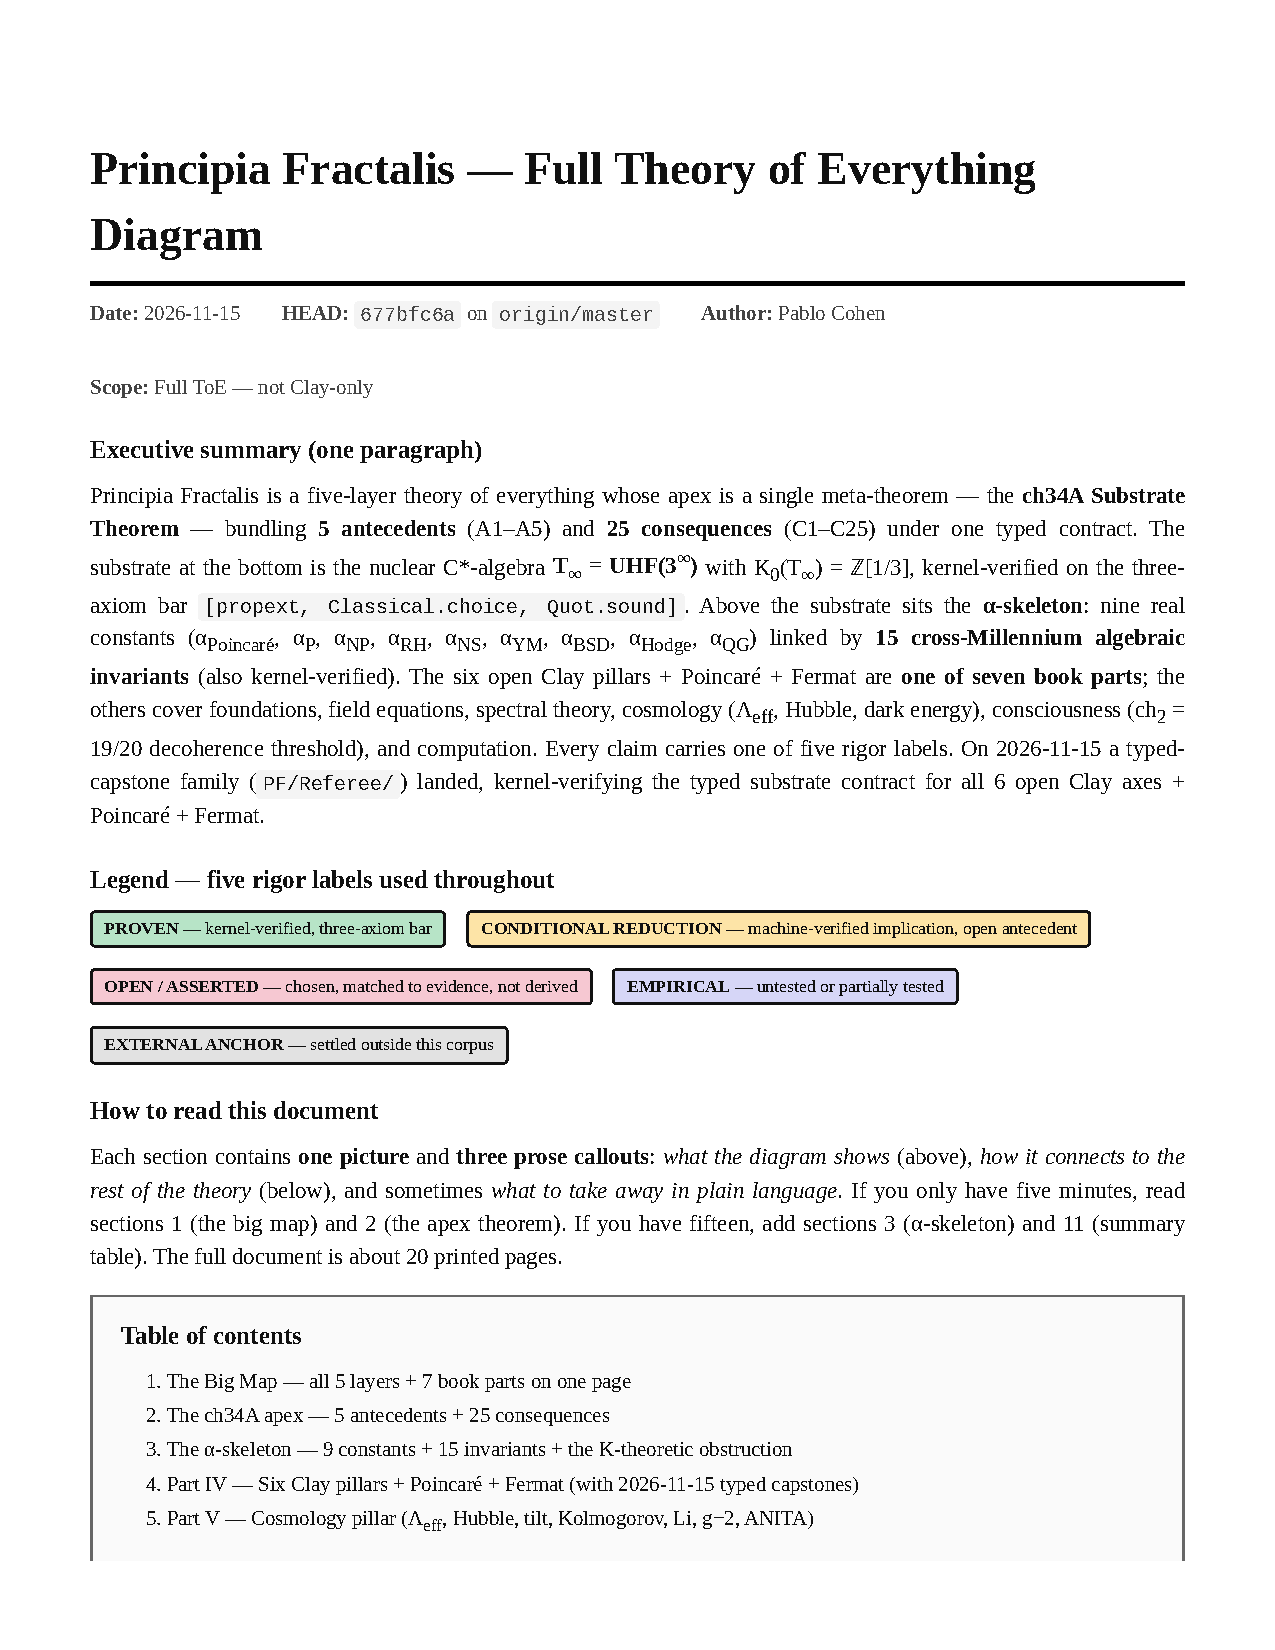
\includepdf[pages=-,pagecommand={\thispagestyle{plain}},fitpaper=true]{figures/pf_toe_diagram_2026_11_15.pdf}
